\begin{figure}[H]
	\centering
	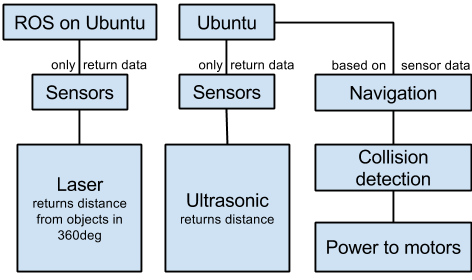
\includegraphics[scale=.7]{images/developmentdiagram2.png}
	\caption{Diagram of the modules we have developed}
	\label{fig:developmentdiagram2}
\end{figure}
%TODO: Elaborate on the figure above

During the initial stages of the project the goal was that we wanted to develop an autonomous mapping vehicle. Unfortunately there were many complications and set-backs preventing us from achieving the original goal. 
 we decided that ROS would be the core of our prototype, because at the time it seemed like the most optimal and most powerful choice for our main operating system. One of the reasons being that there is a lot of documentation and resources about ROS, and people had also previously successfully run ROS and created maps using SLAM on the Raspberry Pi.\cite{pibot}\cite{pibotbook}

Early on in the project we decided that ROS would be the core of our prototype, because at the time it seemed like the most optimal choice for our main operating system. One of the reasons being that there is a lot of documentation and resources about ROS, and people had also previously successfully run ROS and created maps using SLAM on the Raspberry Pi.

The ROS installation process proved to be quite the challenge, which then lead to a setback in terms of development. Many of the ROS packages caused different conflicts with Raspbian operating system, even though these packages should have been compatible with the system out-the-box. After spending too much time on fixing the many errors and getting it to work on Raspbian, we decided to switch to Ubuntu ARM, where the installation process was much easier compared to the previous one.

Using the $I_2C$ interface on the Raspberry Pi we were able to gather measurement data from the Lidar, the next big issue we then encountered was transmitting the gathered data and interpreting it using ROS. Many of the resource regarding gathering data from LIDAR-Lite lasers were mostly regarding USB-based, higher-end devices. %TODO: expand 

%In the beginning of our development period we had some downtime caused by shipping times.

We then at this point realised that we would not have the time and resource to able to make a completely autonomous vehicle, so we instead decided to split the prototype into two separate parts: Navigation and Mapping.\\
What we then aimed to achieve with the laser was to produce a map using SLAM technique. %Add more here, when we know how well it went.

The close proximity detection system, is a low-intelligence autonomous navigation system for the rover. If we succeeded in completing our original scope, the autonomous navigation would have needed to interface with sensors to ensure that it avoided objects at a height that is not recorded by the Lidar and mapping algorithms. So what we have currently achieved is a navigation system that is able to successfully navigate between obstacles by avoiding them and recalculating its direction according to where it detected the obstacles.\\

During testing we observed a couple of key-flaws in terms of the close proximity detection systems performance.
As described in the testing chapter, the rover would at times get stuck in corners due to the equality of the measurements recorded by the ultrasonic sensors. Whenever the ultrasonic sensors mounted on either side of the rover would have their distance threshold exceeded the rover would continuously try to turn to left, hit the one wall of the corner, and then immediately attempt to turn right, hitting the other wall. This can be fixed by changing the code, so that it reverses the rover when the threshold for the side mounted sensors is exceeded. Currently the rover takes three measurements, and then afterwards compares them in the same sequence: \textit{Left > Right > Center}. This unfortunately always prioritizes turning left, compared to other choices. Optimally the code should be structured to that the navigation algorithm consists of multiple phases, so that the rover takes measurements in the first phase and before making a directional decision it compares the measurements to each other in the second phase. When the measurements have been compared, the rover then knows what direction would be the optimal to turn towards, in the third phase the measured distance would be compared to a threshold distance, depending on the return from the comparison the rover would then adjust its direction.
Changing the algorithm to something more similar to the one stated above, would add another level of intelligence to the rover, making it more flexible in terms of navigation and decision-making in other situations.
The rover is currently operated by using four DC motors with regular rubber wheels mounted too them. At this time we do not have precise control of how far the rover moves each time it is powered on.
%TODO: not true, we have encoders on the front wheels for that.
 The rover also does not turn consistently each time, which is either an issue with uneven weight distribution on the rover or because of inaccuracy with the signalling.
To increase the accuracy of the distance moved, encoders for the DC motors can used to determine the distance travelled.
%TODO: this is what I'm talking above.
 In terms of improving how well the rover turns, the rover needs to be balanced and the amount each wheels turns by cycle needs to be determined. Another possible solution for the turning inconsistency is using tracks for movement instead of four independently operated wheels. Tracks would have a larger guarantee %TODO: what?

%TODO:add part about SLAM testing


%TODO:"HOW" the laser mounted on the vehicle works (we basically haven't done this, so it's pure imagination)
Currently, when the mapping device is mounted to the rover, the rover is able to navigating areas whilst the mapping devices creates a map. Due to the low-intelligence of the rover, it is not able to distinguish unknown places from known places, it functions purely by avoiding an object and thereafter determining an optimal direction away from said object.
%TODO:talk about slam integration. 


Too much time during this project was spent chasing the idea of getting SLAM to work. It was a bad combination of tools, because it seems like ROS is made for more advanced computing units, with better interfacing. 
